\documentclass{beamer}
\usepackage{amsfonts,amsmath,oldgerm}
\usepackage{hyperref}
\usepackage[portuguese, brazil, english]{babel}
\usepackage{minted}
\usetheme{sintef}

\hypersetup{
	colorlinks=true,
	linkcolor=white,
	filecolor=blue,      
	urlcolor=blue,
	pdftitle={Aprendendo a Programar em Python - Módulo 01}
}
\newcommand{\testcolor}[1]{\colorbox{#1}{\textcolor{#1}{test}}~\texttt{#1}}

\usefonttheme[onlymath]{serif}

\titlebackground*{assets/background}

\newcommand{\hrefcol}[2]{\textcolor{cyan}{\href{#1}{#2}}}

\title{Introdução ao Python}
\subtitle{Aprendendo a Programar com Python}
\course{Módulo 01}
\author{\href{mailto:augusto.mathias@sesp.pr.gov.br}{Augusto Mathias Adams}}

\begin{document}
\maketitle
\footlinecolor{maincolor}

\begin{frame}

O Nivelamento de \textbf{\textit{Conceitos de Programação - Introdução ao Python }}tem como objetivo introduzir os participantes à linguagem de programação \textit{Python}, fornecendo as habilidades básicas para escrever programas funcionais, compreender conceitos fundamentais e promover a resolução de problemas. Ao final do nivelamento, os alunos estarão preparados para aplicar seus conhecimentos em projetos pessoais ou profissionais.

\end{frame}

\section{Ementa}

\begin{frame}{Pré-requisitos}
	Requisitos mínimos:
	\begin{itemize}
		\item Nenhum conhecimento prévio de programação é necessário.
		\item Um computador com \textbf{\textit{Python}} instalado.
	\end{itemize}
	É desejável:
	\begin{itemize}
		\item \textit{git} instalado (para baixar os exercicios)
		\item Conhecimentos mínimos de \textit{Docker} (será ministrado ao longo do curso)
	\end{itemize}
\end{frame}



\begin{frame}{Conteúdo do Nivelamento}
	O conteúdo deste nivelamento será dividido em 5 partes:
	\begin{itemize}
		\item \textbf{\textit{Módulo 1: }} introdução ao \textit{Python} e princípios básicos de algoritmos.
		\item \textbf{\textit{Módulo 2: }} introdução ao uso de pacotes e programação procedural com \textit{Python} e introdução ao pacote \textit{camera-discovery}.
		\item \textbf{\textit{Módulo 3: }} introdução à programação orientada a objetos e conceitos de banco de dados.
		\item \textbf{\textit{Módulo 4: }} introdução ao \textit{Django} - \textit{Framework} de desenvolvimento web usando python.
		\item \textbf{\textit{Módulo 5: }} produção de um sistema de monitoramento de câmeras usando o pacote \textit{camera-discovery} e \textit{Django}.
	\end{itemize}
\end{frame}

\begin{frame}{Conteúdo do Nivelamento}
	Ao final de cada módulo, será proposta uma lista de exercícios de fixação do conteúdo visto em sala de aula.
\end{frame}

\begin{frame}{Conteúdo do Nivelamento}
	Bibliografia:
	\begin{itemize}
		\item \href{bibliografia/Beginning Programming with Python for Dummies.pdf}{\textbf{\textit{Beginning Programming with Python for Dummies}}}
		\item \href{bibliografia/Algorithms For Dummies.pdf}{\textbf{\textit{Algorithms for Dummies}}}
		\item \href{bibliografia/django-for-beginners-build-websites-with-python-amp-django_compress.pdf}{\textbf{\textit{Django for Beginners}}}
		\item \href{https://django-book.readthedocs.io/en/latest/}{\textbf{\textit{Django Book}}}
		\item \href{https://books.agiliq.com/projects/django-orm-cookbook/en/latest/}{\textbf{\textit{Django ORM Cookbook}}}
		\item \href{bibliografia/The Definitive Guide to Django - Apress.pdf}{\textbf{\textit{The Definitive Guide to Django}}}
	\end{itemize}
\end{frame}

\section{Introdução ao Python}
\subsection{Ementa}
\footlinecolor{maincolor}
\begin{frame}{Objetivos do Módulo}
\begin{itemize}
	\item Do que se trata \textbf{\textit{programar}}.
	\item O que significa o termo \textbf{\textit{algorithmo}}
	\item \textbf{\textit{Sintaxe e Estrutura de Dados}}
	\item \textbf{\textit{Funções em Python}}
	\item Primeira Aplicação em \textbf{\textit{Python}}.
	\item Comentários na sua primeira aplicação.
\end{itemize}
\end{frame}

\subsection{Conceitos De Programação}

\begin{frame}{Conceitos de Programação}

Programar é:

\begin{itemize}
	\item Ato de escrever um conjunto de instruções ou algoritmos que um computador pode executar para realizar uma tarefa específica.
	\item Criação de código em uma linguagem de programação que segue uma sintaxe e estrutura definidas.
	\item Requer habilidades lógicas e analíticas para que as instruções sejam escritas de forma clara e precisa.
\end{itemize}

\end{frame}

\begin{frame}{Conceitos de Programação}
	
	Programar não é:
	
	\begin{itemize}
		\item Falta de planejamento e análise antes de começar a escrever o código.
		\item Ausência de comentários explicativos.
		\item Uso excessivo de linhas de código redundantes ou desnecessária.
		\item Mistura de diferentes estilos e convenções de codificação.
		\item Dificuldade em manter e fazer modificações no código devido à falta de estrutura.
	\end{itemize}
	
\end{frame}

\subsection{Algoritmos}

\begin{frame}{Algoritmo}
	
	Definições:
	
	\begin{itemize}
		\item \textbf{\textit{Algoritmo:}} sequência de passos usada para resolver um problema, fornecendo uma solução específica.
		\item Para ser considerado algoritmo:
		\begin{itemize}
			\item \textbf{\textit{Finito}}: eventualmente resolve o problema. 
			\item \textbf{\textit{Bem definido: }} série de passos precisa e etapas compreensíveis. 
			\item \textbf{\textit{Efetivo: }} resolve todos os casos do problema para o qual foi definido. 
		\end{itemize}
	\end{itemize}
	\alert{\textbf{\textit{Lembre-se:}}} \textbf{\textit{seguindo os passos da receita, conseguimos fazer o bolo!}}
\end{frame}

\begin{frame}{Algoritmos}
\begin{columns}
	\begin{column}{0.5\textwidth}
		\centering
		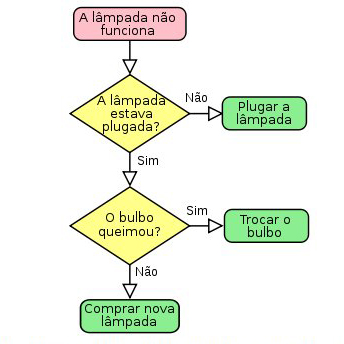
\includegraphics[width=0.7\textwidth]{imagens/fluxograma-exemplo.jpg}
	\end{column}
	\begin{column}{0.5\textwidth}
		\centering
		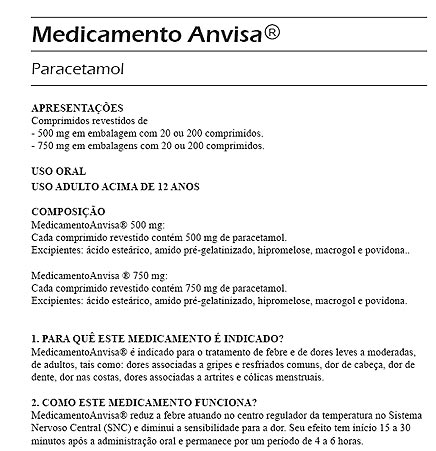
\includegraphics[width=0.7\textwidth]{imagens/nao_e_algoritmo.jpg}
	\end{column}
\end{columns}
\end{frame}

\begin{frame}{Algoritmos}
	Algoritmos comuns (implementados na maioria das linguagens):
	\begin{itemize}
		\item Algoritmos de Busca
		\item Algoritmos de Classificação e Ordenação
		\item Algoritmos de Transformação de Dados
		\item Algoritmos de Agendamento
		\item Algoritmos de Criptografia
		\item Geração de números pseudo-aleatórios
	\end{itemize}
\end{frame}

\section{Linguagem Python}

\subsection{O que é Python}


\begin{frame}{O que é \textit{Python}}
	Do que se trata?
	\begin{itemize}
		\item \textbf{\textit{Definição:}} Linguagem de programação simples e versátil
		\item \textbf{\textit{Características:}}
		\begin{itemize}
			\item 
			\item
			\item 
		\end{itemize}
	\end{itemize}
\end{frame}


\section{Exercícios}

\begin{frame}{Exercício 1 - Algoritmos}
Receita de Bolo da Vovó:
	\begin{itemize}
		\item Pegue uma receita de bolo, ou de qualquer prato que goste (roubar uma receita da esposa serve)
		\item leia atentamente a receita.
		\item descreva utilizando um fluxograma passo a passo a confecção da receita
		\item Dica:
		\begin{itemize}
			\item A receita geralmente é dividida em duas partes: ingredientes e modo de fazer. Inclua os ingredientes como variáveis de entrada. O modo de fazer é, essencialmente, o algoritmo. Divida em quantas partes achar necessário.
		\end{itemize}
	\end{itemize}
\end{frame}

\begin{frame}{Exercício 2 - Algoritmos}
Receita de Bolo da Vovó em \textit{Python}:
\begin{itemize}
	\item Crie uma função para cada item do algoritmo definido no exercício anterior.
	\item Crie uma função que gerenciará os passos de execução do algoritmo.
	\item crie uma chamada de função ao gerenciador que criou e exiba a saída do programa.
	\item \textbf{\textit{Dica:}} copie a estrutura da minha receita contida em \href{Exercicios/Modulo_01/exercicio_01/receita_de_bolo.py}{\textbf{\textit{Receita de Bolo da Vovó}}}
\end{itemize}
\end{frame}


\begin{frame}{Exercício 3 - Algoritmos}
	Implemente um sistema de recomendação para solução de problemas, estilo do algoritmo da lâmpada.
	\begin{itemize}
		\item Não vale utilizar o mesmo exemplo.
		\item Encontre um problema que se resolva em 3 passos na sua casa.
		\item Crie um fluxograma de solução do problema.
		\item Implemente utilizando funções em \textbf{\textit{Python}}, ao estilo do exercício 1.
	\end{itemize}
\end{frame}


\begin{frame}{Exercício 4 - Algoritmos}
	 O que falta na bula de remédios para se tornar um algoritmo? Comente pelo menos 2 casos aplicáveis.
	 
\end{frame}




\backmatter
\end{document}
